\documentclass[pdflatex,sn-mathphys-num]{sn-jnl}% Math and Physical Sciences Numbered Reference Style

%%\documentclass[pdflatex,sn-mathphys-ay]{sn-jnl}% Math and Physical Sciences Author Year Reference Style
%%\documentclass[pdflatex,sn-aps]{sn-jnl}% American Physical Society (APS) Reference Style
%%\documentclass[pdflatex,sn-vancouver-num]{sn-jnl}% Vancouver Numbered Reference Style
%%\documentclass[pdflatex,sn-vancouver-ay]{sn-jnl}% Vancouver Author Year Reference Style
%%\documentclass[pdflatex,sn-apa]{sn-jnl}% APA Reference Style
%%\documentclass[pdflatex,sn-chicago]{sn-jnl}% Chicago-based Humanities Reference Style

%%%% Standard Packages
%%<additional latex packages if required can be included here>
\usepackage{graphicx}
\usepackage{caption}
%\usepackage{subfigure}
\usepackage{subcaption}
\usepackage{booktabs}
\usepackage{longtable}

\usepackage{dsfont}
\usepackage{graphicx}%
\usepackage{multirow}%
\usepackage{amsmath,amssymb,amsfonts}%
\usepackage{amsthm}%
\usepackage{mathrsfs}%
\usepackage[title]{appendix}%
\usepackage{xcolor}%
\usepackage{textcomp}%
\usepackage{manyfoot}%
\usepackage{booktabs}%
\usepackage{algorithm}%
\usepackage{algorithmicx}%
\usepackage{algpseudocode}%
\usepackage{listings}%
%\usepackage{tcolorbox}
\usepackage[most]{tcolorbox}
\usepackage{adjustbox}
\usepackage{array}
\usepackage[utf8]{inputenc}

\usepackage{soul} % \hl{}
\sethlcolor{green!18} % soft highlight; adjust if desired

% Timeline drawing
\usepackage{tikz}
\usetikzlibrary{arrows.meta,positioning}

\usepackage{fancyvrb}      % for Verbatim with inline commands
\usepackage[T1]{fontenc}   % ensures bold typewriter is available
\usepackage{lmodern}       % modern fonts (bold tt)
\usepackage{amsmath}
\usepackage{cleveref}

% Custom margins: left 2in, right 0.75in, top and bottom 1in (consistent on all pages)
\geometry{left=5cm, right=1.5cm, top=1.5cm, bottom=1.5cm, asymmetric}

% Override title page font definitions to use left alignment
\makeatletter

% Redefine fonts to use raggedright instead of titraggedcenter
\def\Titlefont{\reset@font\fontsize{17bp}{22.5bp}\selectfont\raggedright}%
\def\SubTitlefont{\reset@font\fontsize{14bp}{16.5bp}\selectfont\raggedright}%
\def\Authorfont{\reset@font\fontsize{12bp}{14.5bp}\selectfont\boldmath\raggedright}%
\def\addressfont{\reset@font\fontsize{11bp}{13.5bp}\selectfont\raggedright}%
\def\abstractheadfont{\reset@font\fontsize{9bp}{11bp}\bfseries\selectfont\raggedright}%
\def\abstractfont{\reset@font\fontsize{9bp}{11bp}\selectfont\raggedright}%

% Redefine main body text sizes (slightly smaller)
\renewcommand\normalsize{%
   \@setfontsize\normalsize{9.5bp}{11.4bp}%
   \abovedisplayskip 12\p@ \@plus2\p@ \@minus1\p@
   \abovedisplayshortskip \z@ \@plus3\p@%
   \belowdisplayshortskip 3\p@ \@plus3\p@ \@minus3\p@%
   \belowdisplayskip \abovedisplayskip%
   \let\@listi\@listI}%

\renewcommand\small{%
   \@setfontsize\small{8.5bp}{10.2bp}%
   \abovedisplayskip 5\p@ \@plus3\p@ \@minus4\p@
   \abovedisplayshortskip \z@ \@plus2\p@
   \belowdisplayshortskip 3\p@ \@plus2\p@ \@minus2\p@
   \def\@listi{\leftmargin\leftmargini
               \topsep 4\p@ \@plus2\p@ \@minus2\p@
               \parsep 2\p@ \@plus\p@ \@minus\p@
               \itemsep \parsep}%
   \belowdisplayskip \abovedisplayskip}%

\renewcommand\footnotesize{%
   \@setfontsize\footnotesize{7bp}{8bp}%
   \abovedisplayskip 5\p@ \@plus2\p@ \@minus4\p@
   \abovedisplayshortskip \z@ \@plus\p@
   \belowdisplayshortskip 3\p@ \@plus\p@ \@minus2\p@
   \def\@listi{\leftmargin\leftmargini
               \topsep 3\p@ \@plus\p@ \@minus\p@
               \parsep 2\p@ \@plus\p@ \@minus\p@
               \itemsep \parsep}%
   \belowdisplayskip \abovedisplayskip}%

% Redefine section header fonts (smaller)
\def\sectionfont{\reset@font\fontfamily{\rmdefault}\fontsize{12bp}{14bp}\bfseries\selectfont\raggedright\boldmath}%
\def\subsectionfont{\reset@font\fontfamily{\rmdefault}\fontsize{10.5bp}{12.5bp}\bfseries\selectfont\raggedright\boldmath}%
\def\subsubsectionfont{\reset@font\fontsize{9.5bp}{11.5bp}\bfseries\selectfont\raggedright\boldmath}%
\def\paragraphfont{\reset@font\fontsize{9bp}{11bp}\bfseries\itshape\selectfont\raggedright}%

% Reduce top spacing on title page
\renewcommand{\@maketitle}{\newpage\null%
    \if@remarkboxon\vbox to 0pt{\vspace*{-78pt}\hspace*{-18pt}\FMremark}\else\vskip-10pt\fi% Changed from \vskip21pt to \vskip-10pt
    \hsize\textwidth\parindent0pt%
    {\hbox to \textwidth{{\Artcatfont\ArtType\hfill}\par}}%
    \ifx\@title\empty\else%
        \removelastskip\vskip20pt\nointerlineskip%
        {\Titlefont\@title\par}%
    \fi%
    \ifx\@subtitle\empty\else%
        \vskip9pt%
        {{\SubTitlefont\@subtitle\par}}%
    \fi%
    \ifnum\aucount>0
        \global\punctcount\aucount%
        \vskip20pt%
        \artauthors\par%
        {\vskip7pt\addressfont\auaddress\par%
	 \removelastskip\vskip24pt%
	\ifnum\emailcnt>0\relax%
           \ifx\corrauthemail\@empty\else{\ifnum\aucount>1*\fi}%
	   Corresponding author(s). E-mail(s): \corrauthemail\par\fi%
	   \ifx\authemail\@empty\else Contributing authors:\ \authemail\fi%
        \fi%
        \ifequalcont{\par$^{\dagger}$\@equalconttext\par}\fi%
	 \removelastskip\vskip24pt%
        \ifpresentaddress{\par\@presentaddresstext\par}\fi%
	}%
     \fi%
     {\printabstract\par}%
     {\printkeywords\par}%
     \ifx\@pacs\empty\else%
       \loop\ifnum\PacsCount>0%
          \csname\romannumeral\PacsTmpCnt StorePacsTxt\endcsname\par%
          \StepDownCounter{\PacsCount}%
          \StepUpCounter{\PacsTmpCnt}%
       \repeat%
    \fi%
    \removelastskip\vskip36pt\vskip0pt}%

\makeatother

%%%%

%%%%%=============================================================================%%%%
%%%%  Remarks: This template is provided to aid authors with the preparation
%%%%  of original research articles intended for submission to journals published 
%%%%  by Springer Nature. The guidance has been prepared in partnership with 
%%%%  production teams to conform to Springer Nature technical requirements. 
%%%%  Editorial and presentation requirements differ among journal portfolios and 
%%%%  research disciplines. You may find sections in this template are irrelevant 
%%%%  to your work and are empowered to omit any such section if allowed by the 
%%%%  journal you intend to submit to. The submission guidelines and policies 
%%%%  of the journal take precedence. A detailed User Manual is available in the 
%%%%  template package for technical guidance.
%%%%%=============================================================================%%%%

%% as per the requirement new theorem styles can be included as shown below
\theoremstyle{thmstyleone}%
\newtheorem{theorem}{Theorem}%  meant for continuous numbers
%%\newtheorem{theorem}{Theorem}[section]% meant for sectionwise numbers
%% optional argument [theorem] produces theorem numbering sequence instead of independent numbers for Proposition
\newtheorem{proposition}[theorem]{Proposition}% 
%%\newtheorem{proposition}{Proposition}% to get separate numbers for theorem and proposition etc.

\theoremstyle{thmstyletwo}%
\newtheorem{example}{Example}%
\newtheorem{remark}{Remark}%

\theoremstyle{thmstylethree}%
\newtheorem{definition}{Definition}%

\raggedbottom
%%\unnumbered% uncomment this for unnumbered level heads


% %-------------------------------------------------
% % Supplementary Material Formatting for sn-jnl
% %-------------------------------------------------

% \makeatletter

% % Completely suppress the default "Appendix A" title
% \renewcommand\appendix{\par
%   \setcounter{section}{0}%
%   \setcounter{subsection}{0}%
%   \setcounter{subsubsection}{0}%
%   \gdef\thesection{S\arabic{section}}%
%   \gdef\thesubsection{S\arabic{section}.\arabic{subsection}}%
%   \gdef\thesubsubsection{S\arabic{section}.\arabic{subsection}.\arabic{subsubsection}}%
%   \renewcommand{\thefigure}{S\arabic{figure}}%
%   \renewcommand{\thetable}{S\arabic{table}}%
%   \renewcommand{\theequation}{S\arabic{equation}}%
% }

% % Remove the automatic "Appendix" heading inserted by the class
% % \renewcommand\@makechapterhead[1]{}
% % \renewcommand\@makeschapterhead[1]{}

% \makeatother

\begin{document}

\title[Article Title]{Supplementary Material: Temporally annotated textual time series from PubMed Open Access clinical case reports}

%%==================================%%
%% Sample for unstructured abstract %%
%%==================================%%

\maketitle

% Background & Summary
% Methods
% Data Records
% Data Overview (optional)
% Technical Validation
% Usage Notes (optional)
% Data Availability
% Code Availability
% References
% Author Contributions
% Competing Interests
% Acknowledgements (optional)
% Funding
% Ethics statement* 


% \begin{center}
%     {\LARGE Supplementary Material: Temporally annotated textual time series from PubMed Open Access clinical case reports}
% \end{center}
% \vspace{1em} 


\section{LLM Prompts}
\label{apd:llm-prompts}

\input{Scientific_data/Supplementary/TTS_extraction_prompt}
\input{Scientific_data/Supplementary/demo_prompt}
\input{Scientific_data/Supplementary/diagnoses_prompt}


%%%%%%%%%%%%%%%%%%%%%%%%%%%%%%%%%%%%%%%%%%%
%%%%%%%%%%%%%% Evaluation Metrics %%%%%%%%%%%
%%%%%%%%%%%%%%%%%%%%%%%%%%%%%%%%%%%%%%%%%%

\section{Evaluation Metrics}
\label{apd:evaluation-metrics}

We evaluated textual time series extracted from PMOA case reports along three dimensions:
(i) semantic alignment between predicted and manually annotated events (event match rate),
(ii) agreement in temporal ordering (temporal concordance), and
(iii) agreement in timestamp values (time discrepancy).  
Each metric captures a distinct property of timeline quality.

\subsection{Event Match Rate}
\label{apd:event-match-rate}

To assess how well predicted clinical events align with reference events, we use a recursive
best-match strategy adapted from prior work~\cite{wang2025large} as shown in Algorithm~\ref{alg:recursive_match}. At each step, the method
identifies the closest unmatched pair of predicted and reference events using a text-similarity
metric, retains the pair if it satisfies a distance threshold, and removes both events before
proceeding. \textbf{Algorithm \ref{alg:recursive_match}} provides pseudocode for this recursive matching procedure.
This strategy produces a one-to-one alignment between reference and predicted events that is
efficient and well-suited to timelines of differing lengths. 
%\st{Although globally optimal matching methods such as the Hungarian algorithm can be used in principle, they require additional infrastructure to accommodate unequal list sizes and distance thresholds. In practice, the recursive matcher yields assignments nearly identical to optimal solutions while remaining lightweight and interpretable.}

In our final evaluation, we also implement a globally optimal one-to-one matching procedure based on the Linear Assignment Problem, solved using the Jonker–Volgenant (LAPJV) algorithm \citep{jonker1987shortest}. We construct a rectangular cost matrix of pairwise cosine distances between predicted and reference events and enforce a distance threshold by assigning infeasible pairs a prohibitively large cost. LAPJV then computes a minimum-cost assignment under these constraints, yielding a globally optimal one-to-one alignment. This provides a principled benchmark against the recursive heuristic while preserving the same matching constraints. Unlike the recursive best-match heuristic, which greedily selects local minima, the LAPJV formulation optimizes the full matching jointly, ensuring global optimality under the same one-to-one and distance constraints. A detailed sensitivity analysis of LAPJV-based matching with respect to the distance threshold,
including trade-offs between event match rate, temporal concordance, and timestamp accuracy, is presented in Appendix~\ref{apd:lapjv-matching}. 
%\jeremy{This iterative remark is not how the computation works.}


We evaluated several similarity measures—including Levenshtein distance, BERT-based
embeddings, and PubMedBERT embeddings—and found cosine similarity using PubMedBERT
sentence embeddings to perform best. A cosine distance threshold of 0.1 is used to determine
whether a predicted event is considered a semantic match.

Under this procedure, the event match rate is defined as:
\[
\text{Match Rate} =
\frac{\#\{\text{reference events with a matched prediction}\}}
     {\#\{\text{reference events}\}},
\]
which measures the proportion of reference events that are successfully recovered.

\input{Scientific_data/Supplementary/recursive_best_match_algo}


% \begin{table}[ht!]
% \vspace{-3.5mm}
% \centering
% \caption{Bootstrap 95\% confidence intervals for Match Rate, Concordance, and AULTC across models evaluated on the 200 manually annotated case reports.
% %\jeremy{suggest being consistent about number of sigfigs in results (see table 2)}
% }
% \label{tab:bootstrap_intervals}
% \begin{tabular}{lccc}
% \hline
% \textbf{Model} & \textbf{Match Rate (95\% CI)} & \textbf{Concordance (95\% CI)} & \textbf{AULTC (95\% CI)} \\
% \hline
% \texttt{Llama 3.3 70B}      & [0.642, 0.718] & [0.833, 0.861] & [0.701, 0.754] \\
% \texttt{DeepSeek-R1}        & [0.694, 0.773] & [0.783, 0.818] & [0.708, 0.752] \\
% \texttt{DeepSeek-V3-0324}   & [0.727, 0.791] & [0.792, 0.821] & [0.718, 0.758] \\
% \texttt{OpenAI GPT5}        & [0.805, 0.866] & [0.882, 0.898] & [0.706, 0.749] \\
% \texttt{OpenAI O4-mini}     & [0.692, 0.767] & [0.826, 0.852] & [0.732, 0.769] \\
% \texttt{OpenAI O3}          & [0.699, 0.766] & [0.888, 0.907] & [0.728, 0.765] \\
% \texttt{OpenAI O1}          & [0.599, 0.677] & [0.872, 0.895] & [0.716, 0.755] \\
% \hline
% \end{tabular}
% \vspace{-3.5mm}
% \end{table}


\subsection{Temporal Concordance}
\label{apd:temporal-concordance}

Temporal ordering accuracy is quantified using the concordance index (c-index), which
measures the probability that pairs of matched events are ordered correctly in predicted time.
Let $t^{\text{ref}}_i$ and $t^{\text{pred}}_i$ denote the reference and predicted timestamps for
matched event $i$. The c-index is:
\[
\text{c-index} = \frac{1}{N}
\sum_{\substack{i<j\\
t^{\text{ref}}_i \neq t^{\text{ref}}_j\\
t^{\text{pred}}_i \neq t^{\text{pred}}_j}}
\mathds{1}\!\left\{
(t^{\text{ref}}_i - t^{\text{ref}}_j)(t^{\text{pred}}_i - t^{\text{pred}}_j) > 0
\right\},
\]
where $N$ is the number of comparable pairs.  
Higher values indicate stronger preservation of reference ordering.

\subsection{Time Discrepancy and AULTC}
\label{apd:aultc}

For each matched event, we measure timestamp accuracy using the absolute time error
$\Delta t_i = |t^{\text{pred}}_i - t^{\text{ref}}_i|$.  
Because timestamp discrepancies can vary across several orders of magnitude, we evaluate
errors on a log scale:
\[
x_i = \log(1 + \Delta t_i).
\]

To characterize timestamp accuracy across the dataset, we compute the empirical CDF (constructed over log-time discrepancies pooled across all matched events in the 200-case gold standard):
\[
F(x) = \frac{1}{k} \sum_{i=1}^{k} \mathds{1}\{x_i \le x\},
\]
where $k$ is the total number of matched events across all annotated cases.

We then summarize the overall discrepancy using the Area Under the Log-Time CDF (AULTC):
\[
\text{AULTC} =
\frac{1}{\log(1+S_{\max})}
\left[
\sum_{i=1}^{k}(x_{(i)} - x_{(i-1)})\frac{i}{k}
+
\big( \log(1+S_{\max}) - x_{(k)} \big)
\right],
\]
where $x_{(i)}$ are the sorted log discrepancies and $S_{\max}$ is the maximum observed
absolute error.  
AULTC ranges from 0 to 1, with higher values indicating closer alignment between predicted
and reference timestamps.

Finally, we stratify timestamp errors by temporal distance (e.g., within 1 hour, 1 day, 1 week,
1 year) to examine how accuracy varies across clinically meaningful time scales.




%%%%%%%%%%%%%%%%%%%%%%%%%%%%%%%%%%%%%%%%%
%%%%%%%%%%%%% UMLS mapping %%%%%%%%%%%%%%
%%%%%%%%%%%%%%%%%%%%%%%%%%%%%%%%%%%%%%%%

\section{UMLS Mapping for Diagnosis Standardization}
\label{apd:umls-mapping}

To standardize the diagnoses extracted by LLMs from the case reports, we mapped the free-text diagnoses to concepts in the Unified Medical Language System (UMLS). 
This process involved the following steps:

\begin{enumerate}
    \item \textbf{Initial Extraction}: For each case report, we prompted the LLM to extract diagnoses. 
    This yielded a list of free-text diagnoses for each case report.
    \item \textbf{Entity Linking}: We used ScispaCy's entity linker model 
    \texttt{(en\_core\_sci\_lg)} with the UMLS knowledge base to map each extracted diagnosis to corresponding UMLS Concept Unique Identifiers (CUIs). 
    The entity linker identifies potential UMLS concepts and ranks them based on contextual relevance.
    \item \textbf{Filtering and Disambiguation}: For each diagnosis, we:
    \begin{itemize}
       \item Retained only mappings with a confidence score above 0.85
       \item When multiple CUIs were identified for a single diagnosis, selected the highest-ranked mapping
    \end{itemize}
    \item \textbf{Concept Normalization}: After mapping to CUIs, we:
\begin{itemize}
   \item Retrieved the canonical names from UMLS Metathesaurus
   % \item Applied semantic type filtering to ensure mapped concepts were of types relevant to diagnoses (e.g., "Disease or Syndrome", "Pathologic Function", "Mental or Behavioral Dysfunction")
   % \item Grouped synonym concepts where appropriate to reduce redundancy
\end{itemize}
\end{enumerate}

\input{Scientific_data/Supplementary/US_disease_prevalence}

This mapping process allowed us to standardize the diverse expressions of diagnoses extracted by LLMs into a consistent terminology system, enabling more reliable frequency analysis and co-occurrence patterns. 
% \textcolor{red}{Jeremy: Quantify the mapping success rate. Any effects of confidence score or justification for threshold? @Shariar}
Across the full PMOA-TTS corpus, LLM-extracted diagnoses yielded
$N_{\text{raw}} = 63{,}715$ unique free-text diagnosis strings.
Of these, $N_{\text{mapped}} = 41{,}216$ ($64.7\%$) were successfully mapped to at least one
UMLS CUI with a confidence score $\ge 0.85$.
When weighted by frequency of occurrence, mappings at this threshold covered
$91.7\%$ of all diagnosis mentions, indicating that commonly occurring clinical
diagnoses were more likely to receive high-confidence mappings.
Mapping coverage decreased monotonically with increasing confidence threshold.
We therefore selected a threshold of 0.85 as a conservative operating point for
downstream normalization, providing broad coverage of frequently occurring diagnoses
while maintaining a high-confidence mapping criterion.


%%%%%%%%%%%%%%%%%%%%%%%%%%%%%%%%%%%%%%%%%%%
%%%%%%%%%%%%%% Sensitivity analyses %%%%%%%%%%%
%%%%%%%%%%%%%%%%%%%%%%%%%%%%%%%%%%%%%%%%%%

\section{Sensitivity Analyses}
\label{apd:sensitivity-analyses}
%%%%%%%%%%%%%%%%%%%%%%%%%%%%%%%%%%

% \subsection{Varying the Event Match Distance Threshold} %\textcolor{red}{Move to Appendix with figures?}
% \label{sec:choosing_match_threshold}

% We also discuss how adjusting the event match threshold allows tuning the balance between match coverage and ordering accuracy. By varying the event match distance threshold, we obtain different performance characteristics for event match rate, event concordance, and temporal discrepancy (AULTC).  We choose a cosine similarity of 0.1 based on manual review of \texttt{Llama 3.3 70B Instruct} and \texttt{O1} annotations.  Plotting the event match rate versus temporal performance characteristic (concordance and AULTC) when varying the threshold from 0.01 to 0.25, we obtain performance tradeoffs in Figure \ref{fig:threshold_temporal_tradeoff}.

% \begin{figure}
%     \centering
%     % \begin{minipage}{0.45\textwidth}
%         % \centering
%         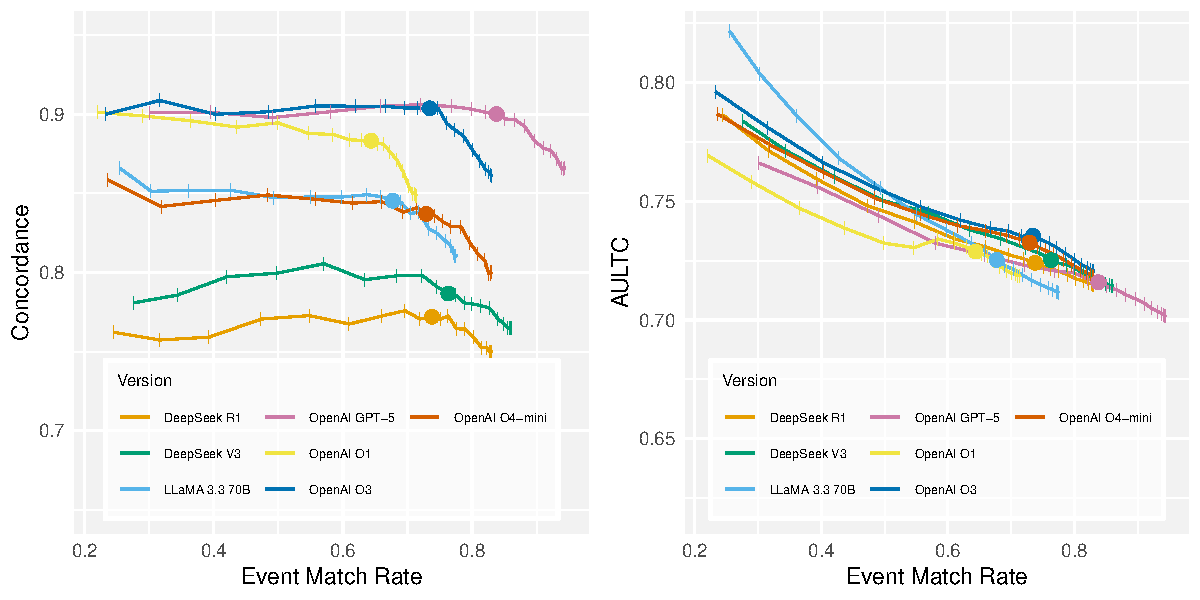
\includegraphics[width=\linewidth]{Plots_tables/event_match_vs_metrics_updated.pdf}
%         % \caption{}
%     % \end{minipage}
%     % \hfill
%     \caption{\textbf{Left:} Concordance by event match rate. Solid circle ($\bullet$) represents threshold of 0.1, with ticks (|) indicating 0.01 increments of the threshold in [0.01, 0.50]. \textbf{Right:} AULTC by event match rate.
%     % \textcolor{red}{Remove \texttt{DSR1-quantized} and replace with \texttt{GPT5}. Rerun on 200?}
%     }
%     \label{fig:threshold_temporal_tradeoff}
% \end{figure}
%%%%%%%%%%%%%%%%%%%%%%%%%%%%%%%%%%%%%%%
\subsection{Sensitivity to Parts of the LLM Prompt Being Changed}
\label{apd:sensitivity-llm-prompt}
%\textcolor{red}{Move to Appendix?}

We slightly modified the prompt from the preceding section to check for sensitivity to specific parts of the LLM prompt being removed or modified.
% For sensitivity analyses with respect to the quality of different prompt strategies for extracting textual time series (\texttt{DeepSeek-R1}) from PMOA case reports, we omitted selected sections of the LLM query prompt
% (see Appendix \ref{apd:extraction_prompt} for the full prompt).
This led to the following variants:
\begin{enumerate}
    \item \textbf{No changes}: Original LLM query prompt. % for \texttt{DeepSeek-R1}.
    
    \item \textbf{No role:} Remove the initial sentence \texttt{"You are a physician."}
    
    \item \textbf{Zero-shot prompting:} Remove the example case report and textual time series from the prompt. \\
    %\item \textbf{No conjunction expansion:} 
    \textcolor{teal}{\texttt{An 18-year-old male was admitted to ...}}\\
    "Let's find the locations of events in the case report, it shows that ... then the output should look like:"\\
    \texttt{18 years old | 0 \\
    male | 0 \\
    ..}

    \item \textbf{No conjunction expansion:} Remove the following sentence from the prompt: \texttt{"Separate conjunctive phrases into their component events and assign them the same timestamp (for example, separation of ‘fever and rash’ into 2 events: ‘fever’ and ‘rash’)"}
    
    \item \textbf{Interval:} A query was added to the prompt for extracting the time interval (start and end time of clinical events). The original prompt’s instructions and few-shot examples were modified accordingly. 
    
    \item \textbf{Interval + Type:} A query was added to the prompt for extracting the time interval and i2b2
    event type (Interval+Type), where event type is one of: Factual, Possible, Hypothetical, Conditional, Negated, Historical, Uncertain. The original prompt’s instructions and few-shot examples were modified accordingly. 
\end{enumerate}

%\input{Scientific_data/Supplementary/prompt_ablation}

\paragraph{Semantic similarity:}
The cumulative distributions of cosine distances between predicted and reference event phrases show clear differences across prompt variants. \emph{Interval} and \emph{Interval+Type} produce the closest matches, while \emph{Zero-shot} performs substantially worse, with a right-shifted distribution indicating lower-quality event spans. \emph{No role} and \emph{No conjunction} show modest degradation relative to the full prompt. These results
demonstrate that including structured temporal guidance and explicit event formatting improves semantic alignment.

\paragraph{Temporal ordering.}
The concordance index (c-index) follows a similar pattern. \emph{Interval+Type} achieves the highest median concordance, followed by \emph{Interval} and the full prompt. Removing role
framing or conjunction splitting reduces ordering consistency, and \emph{Zero-shot} again yields the lowest performance with greater variability. This suggests that structured instructions help the model maintain coherent temporal ordering among extracted events.

\paragraph{Timestamp accuracy.}
Overall log-time discrepancy curves show that \emph{Interval} and \emph{Interval+Type} provide the most accurate timestamp predictions, whereas \emph{Zero-shot} exhibits the largest errors. When stratified by temporal distance from presentation, prompt differences are minimal for
immediate events but widen substantially at longer horizons (1~day, 1~week, 1~year, and beyond). Structured prompts with explicit temporal cues maintain accuracy across these
intervals, while unstructured prompts degrade more quickly.

When stratified by the time from presentation (e.g., within 1 hour, 1 day, 1 week), prompt differences are most pronounced for events occurring farther from the report anchor (Figure \ref{fig:prompt_ablation}, far right). For immediate events, all prompt versions perform comparably. However, at longer timescales (1 week to "ever"), Interval and Interval+Type maintain superior accuracy, while Zero-shot shows dramatic drops in performance. This suggests that structured prompts are particularly critical for accurate long-range temporal reasoning.

Across semantic similarity, temporal ordering, and timestamp alignment, prompt components that provide explicit temporal structure or event-typing requirements consistently improve
performance, while removing instructional scaffolding—particularly in the Zero-shot condition—results in substantial degradation. These findings highlight the importance of prompt
design in guiding LLMs to produce high-quality temporal annotations from clinical narratives.

%%%%%%%%%%%%%%%%%%%%%%%%%%%%%%%%%%%%%%%%%%%

\subsection{Inter-LLM Comparison of Temporal Annotations} 
\label{apd:inter-llm-comparison}
%\textcolor{red}{Move to Appendix?}
%\label{apd:example_annotations}

To illustrate qualitative differences among annotators, we compare temporal event sequences generated by several LLMs for a representative case report (PMC10629858) \citep{abu2023rare}, which describes a patient with lepromatous leprosy who later developed abdominal complications, recurrent bacteremia, severe sepsis, and ultimately died (Figure~\ref{fig:compare_llm_annotations}).

\input{Scientific_data/Supplementary/compare_LLM_TTS_example}

Across models, the principal clinical trajectory is consistently recovered: confirmation of lepromatous leprosy, antibiotic treatment, evolving abdominal symptoms with corresponding imaging findings, subsequent sepsis, ICU readmission, and death. All annotators preserve the
temporal polarity of events, assigning negative times to historical information and positive times to post-admission findings.

Differences emerge in event granularity and phrasing. Some models split conjunctive phrases into multiple events (e.g., listing each component medication separately), whereas others
compress them into single entries. Several annotators also produce near-duplicate events at the same timestamp (e.g., both “diagnosed with lepromatous leprosy’’ and “skin biopsy confirmed’’), reflecting variation in how models segment clinically related information within the narrative.

More pronounced differences appear in temporal normalization. For the expression “two months before admission,” models produce hour offsets ranging from approximately $-1464$ to $-1344$, and one model assigns $-144$ due to an apparent day–hour unit error. Long-range events such as the autologous bone marrow transplant plan, ICU readmission, and death also receive timestamps that vary by hundreds of hours across annotators. Despite this variability in absolute timing,
the relative ordering of major clinical milestones remains largely preserved.

A recurring issue across models involves distinguishing planned actions from events that actually occurred. For example, most annotators correctly represent “planned autologous bone-marrow transplant’’ with an associated future timestamp, which is appropriate because planned interventions can be temporally located and may influence subsequent decision-making. However, several models omit the word “planned,’’ converting the entry into “autologous
bone-marrow transplant’’ and thereby representing an intended but unperformed procedure as an event that occurred. In such cases, the discrepancy arises from the event label rather than the timestamp itself, illustrating how small linguistic omissions can alter the extracted temporal semantics.
%\vspace{-3mm}
\begin{table}[h!]
\centering
\caption{Common error types observed across LLM-generated temporal annotations.}
\label{tab:error_taxonomy}
\begin{tabular}{p{3.2cm} p{9cm}}
\toprule
\textbf{Error Type} & \textbf{Description and Examples} \\
\midrule

\textbf{Event granularity mismatch} 
& Models differ in splitting vs.\ compressing multi-component statements. 
For example, medications may appear as three separate events (``rifampicin'', ``clofazimine'', ``dapsone'') or as one combined entry. \\[6pt]

\textbf{Near-duplicate events} 
& Multiple paraphrased versions of the same clinical concept assigned to the same timestamp, such as 
``diagnosed with lepromatous leprosy’’ and 
``skin biopsy confirmed lepromatous leprosy.’’ \\[6pt]

\textbf{Temporal normalization variability} 
& Large differences in converting narrative expressions (e.g., ``two months before admission’’) to numerical timestamps, with offsets ranging from $-1464$ to $-1344$ hours and occasional scaling errors (e.g., $-144$ hours). Long-range events (e.g., transplant plan, ICU readmission, death) also vary by hundreds of hours across models. \\[6pt]

\textbf{Intent vs.\ occurrence confusion} 
& Some models omit modality markers such as ``planned,'' converting intended future events into events marked as completed. 
The timestamp itself may be reasonable; the error lies in the event label. \\[6pt]

\textbf{Phrasing and specificity variation} 
& Models differ in the level of detail used in event descriptions.  
Some outputs retain clinically precise phrases (e.g., ``mural thickening of the terminal ileum’’), while others produce generic events (e.g., ``abdominal abnormality’’). \\[6pt]

\textbf{Long-range timestamp degradation} 
& Accuracy decreases for events far from the admission anchor, with larger dispersion in timestamp predictions for events weeks or months after presentation. \\
\bottomrule
\end{tabular}
\vspace{-5mm}
\end{table}

Overall, the models capture the broad sequence of events but differ in how they segment conjunctive statements, handle near-duplicates, and resolve absolute times—particularly for
long-range events. A taxonomy of common annotation errors observed across models—including granularity differences, duplicate events, temporal normalization variability, and intent–occurrence misclassification—is summarized in Table~\ref{tab:error_taxonomy}.


\subsection{Sensitivity to Event Matching Strategy (LAPJV)}
\label{apd:lapjv-matching}
We additionally consider a globally optimal one-to-one event alignment based on the Linear Assignment Problem, solved using the Jonker--Volgenant (LAPJV) algorithm \citep{jonker1987shortest}. We define a rectangular cost matrix whose entries are pairwise cosine distances between predicted and reference events. To enforce the same distance thresholding used in the recursive heuristic, we assign a large penalty cost to pairs whose distance exceeds the threshold, effectively masking infeasible matches. LAPJV then computes a minimum-cost assignment under these constraints, yielding a globally optimal one-to-one alignment between the two event sets.

To assess sensitivity to the event alignment procedure, we repeat the inter-LLM comparison using LAPJV-based matching at a cosine distance threshold of 0.1. Table~\ref{tab:model_comparison_lapjv} reports event match rate, temporal concordance, and AULTC across five independent runs per model, and is directly comparable to the main-text results obtained using the recursive matching heuristic (Algorithm~\ref{alg:recursive_match}; Table~\ref{tab:model_comparison}).
% To assess the impact of using a globally optimal matching procedure, we repeat the inter-LLM comparison using LAPJV-based event alignment at a fixed cosine distance threshold of 0.1.
% Table~\ref{tab:model_comparison_lapjv} reports match rate, temporal concordance, and AULTC
% across five independent runs for each model, and is directly comparable to the results obtained
% using the recursive matching heuristic (Algorithm~\ref{alg:recursive_match}) results in Section~\ref{sec:evaluation-of-tts-quality} (Table~\ref{tab:model_comparison}). 
\texttt{OpenAI GPT5} achieves the highest mean match rate (0.850 $\pm$ 0.006), indicating the most comprehensive coverage of manually annotated events. \texttt{OpenAI O3} attains the highest concordance (0.894 $\pm$ 0.004), and \texttt{OpenAI O4-mini} yields the highest AULTC (0.749 $\pm$ 0.003), reflecting strong timestamp alignment among matched events. Standard deviations are generally small across runs, suggesting stable behavior for a given model.


% \begin{table}[!htbp]
% \vspace{-3mm}
% \footnotesize
% \centering
% \caption{Inter-LLM comparison under (top) recursive matching (Algorithm \ref{alg:recursive_match}) and (bottom) LAPJV-based event matching ($\tau = 0.1$), evaluated on 200 manually annotated case reports across five runs per model. \textbf{Best values for each column are marked in bold}.}
% \label{tab:model_comparison_stacked}
% \begin{tabular}{lccc}
% \hline
% \multicolumn{4}{c}{\textbf{Recursive matching (Algorithm \ref{alg:recursive_match})}} \\
% \hline
% \textbf{Model} & \textbf{Match Rate} & \textbf{Concordance} & \textbf{AULTC} \\
% \hline
% \texttt{Llama 3.3 70B}       & 0.675 $\pm$ 0.003 & 0.835 $\pm$ 0.003 & 0.717 $\pm$ 0.001 \\
% \texttt{DeepSeek-R1}         & 0.746 $\pm$ 0.008 & 0.785 $\pm$ 0.010 & 0.726 $\pm$ 0.003 \\
% \texttt{DeepSeek-V3-0324}    & 0.761 $\pm$ 0.004 & 0.791 $\pm$ 0.005 & 0.728 $\pm$ 0.002 \\
% \texttt{OpenAI GPT5}         & \textbf{0.847 $\pm$ 0.005} & 0.883 $\pm$ 0.002 & 0.719 $\pm$ 0.001 \\
% \texttt{OpenAI O4-mini}      & 0.750 $\pm$ 0.019 & 0.842 $\pm$ 0.008 & \textbf{0.748 $\pm$ 0.003} \\
% \texttt{OpenAI O3}           & 0.736 $\pm$ 0.003 & \textbf{0.891 $\pm$ 0.006} & 0.735 $\pm$ 0.003 \\
% \texttt{OpenAI O1}           & 0.638 $\pm$ 0.007 & 0.880 $\pm$ 0.003 & 0.730 $\pm$ 0.001 \\
% \hline
% \multicolumn{4}{c}{}\\[-1.2ex]
% \multicolumn{4}{c}{\textbf{LAPJV matching ($\tau = 0.1$)}} \\
% \hline
% \textbf{Model} & \textbf{Match Rate} & \textbf{Concordance} & \textbf{AULTC} \\
% \hline
% \texttt{Llama 3.3 70B}       & 0.678 $\pm$ 0.003 & 0.838 $\pm$ 0.003 & 0.717 $\pm$ 0.001 \\
% \texttt{DeepSeek-R1}         & 0.749 $\pm$ 0.009 & 0.790 $\pm$ 0.009 & 0.726 $\pm$ 0.004 \\
% \texttt{DeepSeek-V3-0323}    & 0.764 $\pm$ 0.005 & 0.793 $\pm$ 0.007 & 0.728 $\pm$ 0.002 \\
% \texttt{OpenAI GPT5}        & \textbf{0.850 $\pm$ 0.006} & 0.883 $\pm$ 0.003 & 0.719 $\pm$ 0.001 \\
% \texttt{OpenAI O4-mini}      & 0.752 $\pm$ 0.021 & 0.843 $\pm$ 0.008 & \textbf{0.749 $\pm$ 0.003} \\
% \texttt{OpenAI O3}           & 0.739 $\pm$ 0.004 & \textbf{0.894 $\pm$ 0.004} & 0.736 $\pm$ 0.003 \\
% \texttt{OpenAI O1}           & 0.640 $\pm$ 0.008 & 0.881 $\pm$ 0.004 & 0.731 $\pm$ 0.001 \\
% \hline
% \end{tabular}
% \vspace{-3mm}
% \end{table}




\begin{table}[h!]
\vspace{-3mm}
\centering
\caption{Inter-LLM comparison under LAPJV-based event matching (threshold = 0.1), evaluated on 200 manually annotated case reports across five runs per model.}
\label{tab:model_comparison_lapjv}
\begin{tabular}{lccc}
\hline
\textbf{Model} & \textbf{Match Rate} & \textbf{Concordance} & \textbf{AULTC} \\
\hline
\texttt{Llama 3.3 70B}       & 0.678 $\pm$ 0.003 & 0.838 $\pm$ 0.003 & 0.717 $\pm$ 0.001 \\
\texttt{DeepSeek-R1}         & 0.749 $\pm$ 0.009 & 0.790 $\pm$ 0.009 & 0.726 $\pm$ 0.004 \\
\texttt{DeepSeek-V3-0323}    & 0.764 $\pm$ 0.005 & 0.793 $\pm$ 0.007 & 0.728 $\pm$ 0.002 \\
\texttt{OpenAI GPT5}        & \textbf{0.850 $\pm$ 0.006} & 0.883 $\pm$ 0.003 & 0.719 $\pm$ 0.001 \\
\texttt{OpenAI O4-mini}      & 0.752 $\pm$ 0.021 & 0.843 $\pm$ 0.008 & \textbf{0.749 $\pm$ 0.003} \\
\texttt{OpenAI O3}           & 0.739 $\pm$ 0.004 & \textbf{0.894 $\pm$ 0.004} & 0.736 $\pm$ 0.003 \\
\texttt{OpenAI O1}           & 0.640 $\pm$ 0.008 & 0.881 $\pm$ 0.004 & 0.731 $\pm$ 0.001 \\
\hline
\end{tabular}
\vspace{-5mm}
\end{table}


We further examine the trade-off between event match rate and temporal accuracy by sweeping
the LAPJV distance threshold from 0.01 to 0.50 in increments of 0.01. 
Figure~\ref{fig:threshold_tradeoff_LAPJV}
plots temporal concordance and AULTC as a function of event match rate, with the operating
point at threshold 0.1 highlighted.

\begin{figure}[h!]
    \centering
    \includegraphics[width=\linewidth]{Scientific_data/Plots_tables/event_match_vs_metrics_lapjv.pdf}
    \caption{\textbf{A:} Temporal concordance versus event match rate under LAPJV-based matching.
    \textbf{B:} AULTC versus event match rate. Solid circles ($\bullet$) indicate the operating
    threshold of 0.1; ticks (|) denote 0.01 threshold increments in [0.01, 0.50].}
    \label{fig:threshold_tradeoff_LAPJV}
    \vspace{-5mm}
\end{figure}

Across models, LAPJV preserves high event match rates at low thresholds and exhibits a
smooth trade-off between coverage and temporal accuracy. 
The resulting operating points in Figure~\ref{fig:threshold_tradeoff_LAPJV}
are highly comparable to those obtained using the recursive matching heuristic in Figure~\ref{fig:threshold_tradeoff_greedy} (e.g., at $\tau=0.1$, the operating point used in our main results in Table~\ref{tab:model_comparison}). 
In particular,
the heuristic matcher yields slightly stronger concordance near the elbow of the trade-off
curve, while LAPJV achieves marginally higher AULTC values, reflecting improved timestamp
alignment under global assignment. 
Overall, both strategies lead to consistent qualitative
conclusions.




%%%%%%%%%%%%%%%%%%%%%%%%%%%%%%%%%%%%%%%
%%%%%%%%% Survival analysis %%%%%%%%%%
%%%%%%%%%%%%%%%%%%%%%%%%%%%%%%%%%%%%%%%

\section{Survival Analysis Pipeline}
\label{apd:survival-analysis-pipeline}

We developed a survival analysis framework to evaluate the prognostic value of textual information encoded in the time series for time until death prediction. 
Our approach follows a two-stage process:

% \begin{itemize}
%     \item \textcolor{red}{We also did survival for additional open source and medically fine-tuned models}
%     \item \textcolor{red}{Big table and detailed description of methods (task description, models) and results take up too much space. Push most methods in Appendix?. Only describe summarized models in main?}
% \end{itemize}

\begin{enumerate}
\item \textbf{Embedding Extraction}: Each textual time series is converted to a textual context in the format \texttt{"(time) clinical event [SEP] ... [SEP] (time) clinical event [SEP]"} and processed using various pre-trained language models to obtain dense vector representations. 
For encoder models (BERT, RoBERTa, ModernBERT, etc.), we extract the \texttt{[CLS]} token embedding, while for decoder models (\texttt{Llama}, \texttt{DeepSeek-R1}), we compute the mean-pooled embedding over all non-padding tokens.

\item \textbf{Survival Modeling}: These embeddings serve as covariates for two survival models:
\begin{itemize}
    \item \textbf{DeepSurv} \citep{katzman2018deepsurv}: A neural network generalization of the Cox proportional hazards model.
    \item \textbf{DeepHit} \citep{lee2018deephit}: A multi-task neural network jointly modeling discrete hazard and survival functions.
\end{itemize}
\end{enumerate}

We evaluated the performance of the survival models using two metrics: the time-dependent concordance index \citep{antolini2005time}, which measures the model’s ability to correctly rank survival times, and the integrated Brier score (IBS), which captures overall calibration and discrimination over time. 

To ensure reliable estimates, we conducted experiments across five random seeds.
For each seed, we performed a train-validation-test split with proportions of 64\%, 16\%, and 20\%, respectively. 

All survival times were right-censored at a fixed cutoff (\texttt{max\_right\_censoring\_time}=1 year) to maintain consistency across samples. 
Only samples with positive survival times after censoring were included for model training and evaluation.

We tuned hyperparameters independently for each combination of language model and survival model. 
For DeepSurv and DeepHit, we searched over the following hyperparameter grid:
\begin{itemize}
    \item \texttt{num\_nodes}: \{64, 128, 256, 512, 1024, 2048, 4096\}
    \item \texttt{dropout}: \{0.1, 0.5\}
    \item \texttt{epochs}: 2000 (with early stopping)
\end{itemize}

For each configuration, the model was trained on the training set and evaluated on the validation set using the time-dependent concordance index. 
The configuration yielding the highest validation time-dependent concordance was selected, and the corresponding model was then evaluated on the held-out test set. 
This process was repeated for each random seed.
We report the mean and standard deviation of the concordance-index and IBS across the five seeds for each combination of language model and survival model. 

\paragraph{Computational resources:}
For embedding generation in the survival modeling task, decoder models (\texttt{Llama}, \texttt{DeepSeek-R1}) used mean-pooled hidden states, and encoder models (e.g., PubMedBERT) used \texttt{[CLS]} embeddings. Survival models (DeepSurv, DeepHit) were trained using PyTorch on single NVIDIA GeForce RTX 4090. Each training run optimizing across the hyperparameter grid for the validation set took on average 195 minutes. Hyperparameter search across seeds, dropout values, and hidden node counts resulted in 48 GPU-hours total compute.

\bibliography{Scientific_data/references}



%%===========================================================================================%%

\end{document}
